
%%%%%%%%%%%%%%%%%%%%%%% file typeinst.tex %%%%%%%%%%%%%%%%%%%%%%%%%%%%%%
%
% This is the LaTeX source for the instructions to authors using
% the LaTeX document class SVMultln with class option 'lnicst'
% for contributions to the Lecture Notes of the Institute for
% Computer Sciences, Social-Informatics and
% Telecommunications Engineering series.
% www.springer.com/series/XXXX       Springer Heidelberg 2007/08/05
%
% It may be used as a template for your own input - copy it
% to a new file with a new name and use it as the basis for
% your article. It contains a few tweaked sections to demonstrate
% features of the package, though.
%
% If you have not much experiences with Springer LaTeX support,
% you should better use the special demonstration file "lnicst.tex"
% included in the LaTeX package for LNICST as template.
%
%%%%%%%%%%%%%%%%%%%%%%%%%%%%%%%%%%%%%%%%%%%%%%%%%%%%%%%%%%%%%%%%%%%%%%%%

\documentclass[lnicst,sechang,a4paper]{svmultln}
\usepackage{amssymb}
\setcounter{tocdepth}{3}
\usepackage{graphicx}

\usepackage{url}
\urldef{\mailsa}\path|{mohsin.khan, valtteri.niemi}@helsinki.fi|
\usepackage[pdfpagelabels,hypertexnames=false,breaklinks=true,bookmarksopen=true,bookmarksopenlevel=2]{hyperref}


%added by the author himself
\usepackage{color}
\usepackage[numbers]{natbib}
\usepackage{calc}
\usepackage{siunitx}
\DeclareSIUnit\mt{\milli\tesla} %% A method for say short cut or new unit!
\sisetup{inter-unit-product = {-}}

\begin{document}

\mainmatter  % start of an individual contribution

% first the title is needed
\title{AES and SNOW 3G are Feasible Choices for a 5G Phone from Energy Perspective}

% a short form should be given in case it is too long for the running head
\titlerunning{AES and SNOW 3G are Feasible Choices}

% the name(s) of the author(s) follow(s) next
%
% NB: Chinese authors should write their first names(s) in front of
% their surnames. This ensures that the names appear correctly in
% the running heads and the author index.
%
\author{Mohsin Khan%
%%\thanks{Please note that the LNICST Editorial assumes that all authors have used
%%the western naming convention, with given names preceding surnames. This determines
%%the structure of the names in the running heads and the author index.}%
\and Valtteri Niemi}  %
%\authorrunning{Lecture Notes of ICST: Authors' Instructions}
% (feature abused for this document to repeat the title also on left hand pages)

% the affiliations are given next
\institute{University of Helsinki, Department of Computer Science,\\
P.O. Box 68 (Gustaf H\"allstr\"amin katu 2b)\\
FI-00014 University of Helsinki\\
Finland\\
\mailsa
%\\
%\url{http://www.springer.com/series/7911}
}

%
% NB: a more complex sample for affiliations and the mapping to the
% corresponding authors can be found in the file "lnicst.dem",
% that is contained in the LNICST LaTeX support package.
%

\toctitle{AES and SNOW 3G are Feasible Choices}
\tocauthor{Authors' Instructions}
\maketitle


\begin{abstract}
The aspirations for a 5th generation (5G) mobile network are high. It has a vision of unprecedented data-rate and extremely pervasive connectivity. To cater such aspirations in a mobile phone, many existing efficiency aspects of a mobile phone need to be reviewed. We look into the matter of required energy to encrypt and decrypt the huge amount of traffic that will leave from and enter into a 5G enabled mobile phone. In this paper, we present an account of the power consumption details of the efficient hardware implementations of AES and SNOW 3G. We also present an account of the power consumption details of LTE protocol stack on some cutting edge hardware platforms. Based on the aforementioned two accounts, we argue that the energy requirement for the current encryption systems AES and SNOW 3G will not impact the battery-life of a 5G enabled mobile phone by any significant proportion.
\keywords{5G $\cdot$ Cryptosystem $\cdot$ ASIC}
\end{abstract}


\section{Introduction}
\label{intro} To facilitate our discussion, we need to know what are the data that will be encrypted and decrypted in a 5G phone. We also need to know where and how many times the encryption and decryption will take place across the protocol stack on the phone. But 5G is not yet a reality and we do not have exact answers to these questions. So, we assume things, that will be true for a 5G network and argue on the basis of those assumptions. We turn to the LTE network to make the assumptions. In an LTE phone, the data that leave and enter the phone can be broadly classified into three categories. The first one are the control signals in between the phone and the core network. The second one are the control signals in between the phone and the radio network. And t
\label{sec:aes}he third one are the user data which the user sends and receives at the phone's application layer. Both of the first two categories are privacy and integrity protected. For the third category, only the privacy is protected. Also note that, from the volume point of view, the major share of data belong to the third category. Comparing to the the third category, the cryptographic computational need required for the data of first and second categories is negligible. The user data in an LTE phone is only once encrypted and decrypted across the protocol stack in PDCP layer. In an LTE phone this encryption is done by an application specific integrated circuit (ASIC).

For a 5G phone, we assume that the user data will remain as the major share of the total data leaving and entering the phone. The cryptographic computational need for the total volume of control signals will be negligible in comparison with that of the user data. The user data will only once be encrypted and decrypted somewhere across the protocol stack. From hardware point of view it will still be in an ASIC. In order to have a pessimistic estimation, we assume that integrity protection of user data will be introduced in 5G. Based on these assumptions, we will look into the cryptographic energy requirements and also the total energy requirements across the whole protocol stack of an LTE phone. Then we will scale up the data-rate from 100 Mbps to 1 Gbps and see how much extra pressure it puts on the battery of the phone in comparison with other energy hungry aspects of the phone like display and radio signalling.

The paper is organized by first giving a very short introduction to the architecture, the protocol stack and the cryptographic specifications of the LTE network in section \ref{sec:lte_specifications}. In section \ref{sec:throughput_and_energy_requirements_of_aes_snow3g}, we present the experimental results about the energy requirements of the two cryptosystems of interest, which are AES and SNOW 3G. In this section we also present the experimental result about the energy consumption across the whole protocol stack of the link layer. In section \ref{sec:overall_comparison} we present the energy consumption distribution of the whole phone among it's different functional modules and show that the energy needed for cryptographic computation is not a threat for the battery life of the phone. 

\section{LTE specifications}
\label{sec:lte_specifications}
An LTE network is comprised of broadly three components. The user equipment (UE), evolved radio network (E-UTRAN) known as radio network and evolved packet core (EPC) known as core network. The user equipment consists of a mobile equipment (ME) or a mobile phone for the context of this paper, and an universal integrated circuit card (UICC). The UICC hosts an application called subscriber identification module (SIM). In this paper when we refer to the user equipment, we mean it to be the mobile phone since the UICC does not have much functionality to consume a lot of energy.

\begin{figure}
% Use the relevant command to insert your figure file.
% For example, with the graphicx package use
  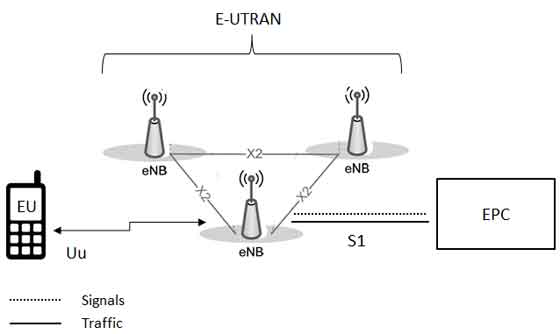
\includegraphics[width=0.95\textwidth]{lte_architecture.jpg}
% figure caption is below the figure
\caption{LTE Architecture, it is a dummy figure, I will draw my own figure}
\label{fig:protocl_stack}       % Give a unique label
\end{figure}

The UE is connected to the network via a radio link only with the radio network. The entity of the E-UTRAN that has the radio link with the UE is called eNodeB which is tradionally known as a base station. However, the UE also establishes a direct logical connection with an entity of the core network known as mobility management entity (MME). This logical connection is used only for the control signals for the core network and hence we do not focus on it in this paper. The user data as mentioned in the introduction travels from the UE to the eNodeB. Figure \ref{fig:protocl_stack} shows the protocol stack that the data travel across at the UE and at eNodeB. The L1 layer is the physical layer. We logically bundle the PDCP, RLC and MAC layers as layer 2 (L2) layer. All the encryption and decryption takes place at the PDCP layer \cite{3GPP_TS_36_323}.

\begin{figure}
% Use the relevant command to insert your figure file.
% For example, with the graphicx package use
  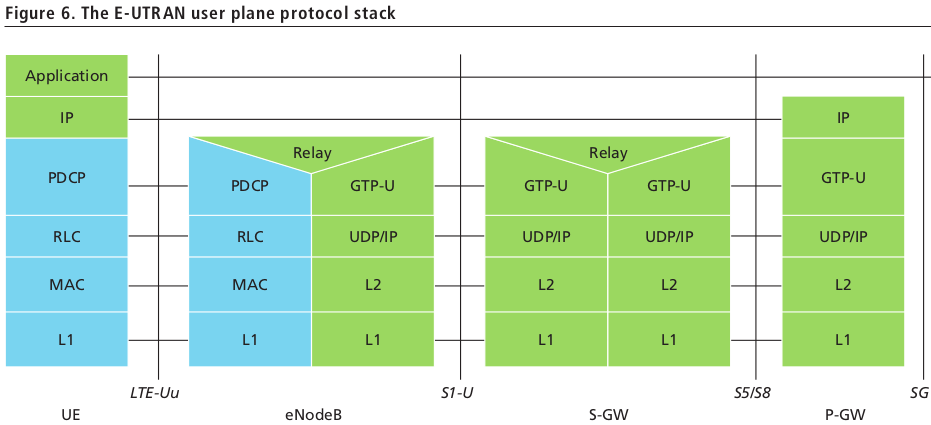
\includegraphics[width=1\textwidth]{protocl_stack.png}
% figure caption is below the figure
\caption{Protocol stack, it is a dummy figure, I will draw my own figure}
\label{fig:protocl_stack}       % Give a unique label
\end{figure}

According to \cite{3GPP_TS_33_401}, there are two mandatory sets of security algorithms in the 4th generation cellular network (LTE) developed by 3GPP. One is EEA1 in which the stream cipher SNOW 3G is used. The other is EEA2 in which the block cipher AES is used. The aspiration about 5G networks is to obtain at least 1Gbps data-rate. The question arises, if there are implementations of these two encryption systems that can achieve the required throughput and still be enough energy efficient to use in a mobile phone.

\section{Throughput and energy requirements of AES and SNOW 3G}
\label{sec:throughput_and_energy_requirements_of_aes_snow3g}
In \cite{IIS_Ruhr_2009}, the authors in their experiment showed that the computing power of a single embedded processor at reasonable clock frequencies is not enough to cope with the L2 requirements of LTE and next generation mobile devices. They illustrated that a conventional hardware acceleration approach for the encryption algorithms fail to offer the performance required by LTE and future mobile devices. The AES decryption was identified as the major time critical software algorithm, demanding half of the entire L2 DL execution time. So, more advanced hardware acceleration methods were required while keeping the energy and area requirement at a reasonable level for a mobile phone.

In \cite{IIS_Ruhr_2010}, a study conducted on the L2 DL (MAC, PDCP, RLC) layer, the authors have shown that by a smart DMA (direct memory access) controller, the required throughput for LTE which is at most 100 Mbps can be achieved. However, to achive this required throughput, the implementation consumed 9.5 mW of power whereas AES and SNOW 3G each required .5 and .57 mW of power respectively. Which means the decryption consumes around 5 percent of the power budget of L2 DL. From energy point of view, it consumes 5.7 mJ of energy to decrypt one giga bit of data. The area effort is also only 15 percent of the total requirement of L2 DL. The figure 6 and 8 in \cite{IIS_Ruhr_2010} presents the detailed comparison. In section \ref{sec:overall_comparison}, we will see that this is indeed a very small amount of energy when compared with total amount of energy consumed by the phone while exchanging bulk amount of network data.

We see ciphering is not very expensive in LTE. But it needs to be rigorously investigated to conclude that it will not be very expensive in 5G. Because, from our experience of LTE, we see that the energy requirements of radio interface technology in LTE does not increase linearly with the data rate but energy requirements for encryption is almost linear to the size of the data being encrypted. 5G has unprecedented data rate of 1Gbps and we need to show that even such a bulk volume of encryption doesn't incur much energy when compared with the total energy spent. In the following sub-sections we present some implementations of AES and SNOW 3G.

\subsection{AES} Since the adoption of Rijndael as AES by NIST, there have been a number of hardware implementations of AES. In the beginning, the focus was completely on achieving high throughput. Nevertheless, over the time the need for energy efficient implementations became more pressing and we found the following result available in the literature. \newline


\begin{table}
\begin{center}
\begin{tabular}{|p{0.16\textwidth-2\tabcolsep}
				|p{0.08\textwidth-2\tabcolsep}
				|p{0.16\textwidth-2\tabcolsep}
				|p{0.2\textwidth-2\tabcolsep}
				|p{0.18\textwidth-2\tabcolsep}
				|p{0.16\textwidth-2\tabcolsep}|
				}
\hline
Year & Ref & TP (Gbps) & Gates(K) & Power (mW) & Energy (mJ/Gb) \\
\hline
2001 & \cite{IBM_Japan_2001} &$2.6$ &$21.3$  & $-$ & $-$ \\ \hline
2001 & \cite{IBM_Japan_2001} &$.311$ &$5.4$  & $-$ & $-$ \\ \hline
2001 & \cite{IBM_India_IIT_2001} &$.24$ &$4$  & $-$ & $-$ \\ \hline
2006 & \cite{Taiwan_2006} &$.570$ & - &20.34 & 35.68 \\ \hline
2006 & \cite{Taiwan_2006} &$.569$ & - &192.5 & 33.83 \\ \hline
2007 & \cite{IIT_Kharagpur_2007} &$.384$ &$21$ & $-$  & $-$ \\ \hline
2009 & \cite{IME_China_Tsinghua_Univerisity_2009} &$1.16$ &$19.47$ & $-$ & $-$ \\ \hline
2009 & \cite{Ruhr_2009} &$\geq 1.00$ &$38$ &1.18 & $\leq 1.18$ \\ \hline
2011 & \cite{Ruhr_2011} &$.114$ &$ - $ &.02 & .24 \\ \hline
2012 & \cite{Pune_2012} &$1.6$ &$58.445$ &22.85 & 14.28 \\ \hline
\end{tabular}
\end{center}
\caption{AES Implementations}
\label{table:aes_implementation}
\end{table}

From Table \ref{table:aes_implementation}, we find the implementations in \cite{Ruhr_2009}, \cite{Ruhr_2011}, \cite{Pune_2012} are potential candidates for using in 5G. Because they meet the required throughput of 5G and present their energy requirements which enable us to make a meaningful argument. In \cite{Ruhr_2009}, the authors doesn't provide the exact throughput but say that it achieves at least $1$ Gbps by using multi-AES architecture. In \cite{Ruhr_2011}, the authors present an implementation (SAME) that achieves $.114$ Gbps throughput using $2$ cores which they claim to be scalable with a speed up factor of $.84$. According to figure 9 in \cite{Ruhr_2011}, the SAME implementation achieves $5.5$ Mbps/$\mu$J. Which means it spends $114/5.5 = 20.72$ $\mu$J $=.02$ mJ to encrypt/decrypt $114$ Mbit. Now, by scaling up by $12$ different $2$-cores, it will achieve the throughput of $.114 \times 12 \times .83 = 1$ Gbps while it will spend $.02*12=.24$ mJ $=.24$ mJ. In \cite{Pune_2012}, the implementation achieves the required throughput without any need of scaling up and it spends comparatively high energy than that of \cite{Ruhr_2009} and \cite{Ruhr_2011}. 

In the next section, we make an overall comparison to see how much these numerical values matter in the context of the energy requirements for the whole mobile phone. To make an overall comparison, we choose the implementation in \cite{Ruhr_2011} because it has the best energy figure. However, the comparison with the implementation in \cite{Ruhr_2009} can also be easily presented as it is simply $5$ times more energy-expensive than that of \cite{Ruhr_2011}. It appears that the implementation in \cite{Pune_2012} is $60$ times more expensive than that of \cite{Ruhr_2011}. So, we exclude it from our consideration. 

\subsection{SNOW 3G}
\label{sub-sec:snow3gp}
More text will come in

\section{Overall comparison}
\label{sec:overall_comparison}
The overall energy consumption of a phone depends on the usage type of the user of the phone. Radio activities of the cellular network, lighting up the screen, touch screen and CPU are the commonly known energy hungry aspects of a smart phone \cite{Usenix_2010}. 

There are times when a smart phone remains idle and does nothing for a long duration of time. During this time it moves to a suspended state by transferring the state of the phone to the RAM. In suspended state the phone draws a minimal amount of energy from the battery to maintain the state in the memory and receive very limited control signals from the network to be able to receive the incoming traffic. In \cite{Usenix_2010}, the authors conducted an experiment on a $2.5$G phone and two cutting edge $3$G phones of the time. They showed that in suspended state, the $2.5$G phone draws $103$ mJ of energy per second whereas the 3G phones draw around $25$ mJ per second. There is another state when the phone is awake but no application is running. This state is called the idle state. In \cite{Usenix_2010}, the authors showed on the same phones that during idle state the amount of energy drawn is less than $350$ mJ per second. 

Normally, the time duration of a smart phone when it remains suspended or idle is much longer than that of when it remains active. So, the energy consumption of the phone during idle or suspended state is very critical for the battery life. However, during these times, the phone hardly encrypts or decrypts any data except the control signals which are mostly paging messages. Because attach procedure takes place only when the user switches on the phone and tracking area update takes place frequently only when the user is travelling on a vehicle. However, even though paging itself is a burden for the phone from energy point of view, the cryptographic energy requirement for paging message is insignificant. According to \cite{Nokia_2013}, even with traditional paging mechanism, there are $1000$ paging messages for a phone in an hour, which is less than $1$ in a second. And according to \cite{3GPP_TS_36_331}, the paging message is no longer than hundreds of bytes. The energy requirements for AES for this tiny amount of data is very insignificant to the total need $25$ mJ per second during the suspended state and of 300 mJ during the idle state.

To understand the energy expense of encryption, we need to focus on the total energy expense of the phone during the active states of the phone when encryption is also being performed. Such active states are phone call, web browsing, email, network data exchange (upload/download) and so on. We choose the case of network data exchange to argue our case. We assume that the phone would exhaust it's full download or upload capacity from the data volume point of view during the exchange. We will investigate this case for 2.5G, 3G and 4G phones to see the evolution the energy requirements.

In \cite{Usenix_2010}, the authors showed that the $2.5$G phone consumed around $700$ mJ of energy per second during the network data exchange. Around $640$ mJ of this energy budget is spend for cellular network activities. We know in $2.5$G, the maximum data rate can be 115 Kbps. In that rate AES implementation in \cite{Ruhr_2011} would spend around $.000024$ mJ of energy per second which is of course very insignificant. The authors of \cite{Usenix_2010} also showed that the 3G phones consumed similar amount of total energy during the data upload/download which is around $900$ mJ. We consider that the connection exchanged the data at its full capacity (which is 7.2 Mbps), the energy share for encryption is around $0.002$ mJ which is also very insignificant. 

Both in the 2.5G and 3G phone the major energy share for network data exchange is attributed to the radio transmission. However, there has been a significant change in the LTE radio technology and has become even more expensive from energy consumption point of view. In LTE, there are different radio states and the phone promotes and demotes to different states to save energy. As a result even though LTE become less energy efficient than 3G for small data transfer, it remains as efficient as 3G in large size data transfer. Also, there is significant difference in the energy consumption of LTE uplink and downlink. According to \cite{Mobisys_2012}, the LTE uplink consumes $3.2$ J of energy per second whereas uploading at a rate of $1$ Mbps consumes $2.1$ J of energy per second. With screen off, the authors claimed that the energy was mostly consumed by the radio interfaces. The AES implementation in \cite{Ruhr_2011} consumes $.24$ mJ of energy per second providing throughput of $1$ Gbps. So, the energy share of of encryption is less than .0004 percent of the total requirement. Very optimistically if we consider that the LTE transmission would consume the same amount of energy even when the data rate is at the theoretical peak which is 100 Mbps, the energy share of encryption is still bounded by $.01$ percent. It should be noted here that the high energy requirements in LTE is mostly attributed to it's radio interface technology. Nevertheless, the radio technology will be different in 5G than that of LTE. Let us consider that the LTE draws $E_{lte}$ mJ of energy per second while transferring data at 100 Mbps. Let's assume that in 5G, the radio interface will draw $E_{lte}/a$ mJ of energy while providing throughput of $1$ Gbps by using it's new efficient radio technology, if there is any. And we know implementation of AES that takes $.24$ mJ of energy per second to provide throughput of $1$ Gbps. So, the energy share of encryption in 5G is $\frac{.24a}{E_{lte}}\times 100 = .01a$ percent

\section{Conclusion}
\label{sec:conclusion}
I will wrtie the conclusion later

\section{Acknowledgement}
\label{sec:acknowledgement}
??


\begin{thebibliography}{4}

\bibitem{3GPP_TS_36_323} 3GPP TS36.323, http://www.3gpp.org/ftp/specs/archive/36\_series/36.323/
\bibitem{3GPP_TS_33_401} 3GPP TS33.401, http://www.3gpp.org/ftp/specs/archive/33\_series/33.401/
\bibitem{3GPP_TS_36_331} 3GPP TS36.331, http://www.3gpp.org/ftp/specs/archive/36\_series/36.331/

\bibitem{IBM_Japan_2001} Akashi Satoh, Sumio Morioka, Kohji Takano, Seiji Munetoh: A Compact Rijndael Hardware Architecture with S-Box Optimization. In: LNCS, Advances in Cryptology — ASIACRYPT 2001, pp. 239--254. Springer (2001)


\bibitem{IBM_India_IIT_2001} Atri Rudra, Pradeep K. Dubey, Charanjit S. Jutla, Vijay Kumar, Josyula R. Rao, Pankaj Rohatgi: Efficient Rijndael Encryption Implementation with Composite Field Arithmetic. In: LNCS, Cryptographic Hardware and Embedded Systems — CHES 2001, pp. 171--184. Springer (2001)


\bibitem{IME_China_Tsinghua_Univerisity_2009} Qingfu Cao, Shuguo Li: A high-throughput cost-effective ASIC implementation of the AES Algorithm. 2009 IEEE 8th International Conference on ASIC (2009)


\bibitem{IIT_Kharagpur_2007} Monjur Alam, Sonai Ray,	Debdeep Mukhopadhayay, Santosh Ghosh,  Dipanwita RoyChowdhury, Indranil Sengupta: Efficient Rijndael Encryption Implementation with Composite Field Arithmetic. In: Proceedings of the conference on Design, automation and test in Europe
 — DATE'07, pp. 1116--1121. Springer (2007)


\bibitem{Taiwan_2006} Yu-Jung Huang, Yang-Shih Lin,  Kuang-Yu Hung, Kuo-Chen Lin: Efficient Implementation of AES IP. 2006 IEEE Asia Pacific Conference on Circuits and Systems (2006)

\bibitem{Ruhr_2009} Sebastian Hessel, David Szczesny, Nils Lohmann, Attila Bilgic, Josef Hausner: Implementation and Benchmarking of Hardware Accelerators for Ciphering in LTE Terminals. Global Telecommunications Conference, 2009 (2009)

\bibitem{Ruhr_2011} SShadi Traboulsi, Mohamad Sbeiti, David Szczesny, Anas Showk, Attila Bilgic: High-performance and energy-efficient sliced AES multi-block encryption for LTE mobile devices. 2011 IEEE 3rd International Conference on Communication Software and Networks (2001)


\bibitem{Pune_2012} P. V. Sriniwas Shastry, Amruta Kulkarni, Mukul S. Sutaone: ASIC implementation of AES. 2012 Annual IEEE India Conference  (2012)

\bibitem{IIS_Ruhr_2009} David Szczesny, Anas Showk, Sebastian Hessel, Attila Bilgic, Uwe Hildebrand, Valerio Frascolla: Performance analysis of LTE protocol processing on an ARM based mobile platform. International Symposium on System-on-Chip, 2009 (2009)


\bibitem{KTH_2014} Mohammad Badawi, Ahmed Hemani, Zhonghai Lu: Customizable coarse-grained energy-efficient reconfigurable packet processing architecture. 2014 IEEE 25th International Conference on Application-Specific Systems, Architectures and Processors (2014)

\bibitem{IIS_Ruhr_2010} Sebastian Hessel, David Szczesny, Felix Bruns, Attila Bilgic, Josef Hausner: Architectural Analysis of a Smart DMA Controller for Protocol Stack Acceleration in LTE Terminals. Vehicular Technology Conference Fall (VTC 2010-Fall), 2010 IEEE 72nd (2010)


\bibitem{Usenix_2010} Aaron Carroll, Gernot Heiser: An analysis of power consumption in a smartphone. USENIXATC'10 Proceedings of the 2010 USENIX conference on USENIX annual technical conference (2010)


\bibitem{Mobisys_2012} Junxian Huang, Feng Qian, Alexandre Gerber, Z. Morley Mao, Subhabrata Sen, Oliver Spatscheckr: A close examination of performance and power characteristics of 4G LTE networks. Proceedings of the 10th international conference on Mobile systems, applications, and services (2012)

\bibitem{Nokia_2013} Managing LTE Core Network Signaling Traffic by David Nowoswiat, https://insight.nokia.com/managing-lte-core-network-signaling-traffic

\end{thebibliography}

\end{document}
